\chapter{Appendix}\label{append}

% \section{Anderson-Darling statistic}\label{app_ad}

% Two-sample Anderson - Darling statistic is~defined as:

% \begin{equation}
% \label{two-sample_ad}
%   A^2_{nm}=\frac{mn}{N} \int\limits_{-\infty}^{\infty} \frac{\{F^i_m(x) - F^j_n(x) \}^2} {H_N(x)(1-H_N(x))}dH_N(x),
% \end{equation}

% where $F^i_m$, $F^j_n$ are empirical cumulative distribution functions of~$i^{th}$ and $j^{th}$ data sets, and $H_N$ with $N=n+m$ is~the~weight function, for $n$ and $m$ being the~number of~observations in~data sets. The $H_N$ function is~given by~combining $F^i_m$ and $F^j_n$ distribution: $H_N(x)=\frac{mF^i_m(x)+nF^j_n(x)}{N}$. It is~used to~test hypothesis $F^i_m=F^j_n$.




\section{Short-Time Fourier Transform}\label{STFT}

Author have used Short-Time Fourier transform (STFT) as~a~beginning point in~most of~the~analysis. It is~one of~the~most useful time-frequency decompositions. We define this transform as~\cite{allen1977short}:
\begin{equation}
STFT(t,f)=\int_{-\infty}^{\infty} X(\tau) w(t-\tau) e^{2 j \pi f \tau}
\end{equation}

Its discrete form is~defined as:
\begin{equation}
STFT(t,f)=\sum_{k=1}^{n} x[k] w(t-k) e^{\frac{2 j \pi f k}{n}},
\end{equation}
where $w(t-k)$ is~the~shifting window and $x_k$ is~the~discrete signal $(k=1,2,...n)$.

It allows one to~track energy changes through both time and frequency. It is~widely known that impulsive behavior will produce series of~high-energy excitations and thus, spectrogram (squared absolute value of~the~STFT) can point them out in~its graphical representation. We define spectrogram as:
\begin{equation}
spec(t,f)=|STFT(t,f)|^2
\end{equation} 

\section{Silhouette criterion}\label{app_sil}

Silhouette criterion is~a~widely known and one of~the~simplest measures of~clustering quality \cite{rousseeuw1987silhouettes}. Assume data set clustered into $k$ clusters. For every data point $i \in C_i$ (data point $i$ in~cluster $C_i$), let us define

\begin{equation}
  a(i)=\frac{1}{|C_i|-1}\sum_{j\in C_i, i\neq j}d(i,j)
\end{equation}
to be~the~average distance between $i$ and every other data point in~the~same cluster, where $d(i,j)$ is~the~distance between points $i$ and $j$ in~the~cluster $C_i$, and division by~$|C_i|-1$ takes into consideration that distance $d(i,i)$ is~not included in~the~sum. This way $a(i)$ can be~interpreted as~the~measure of~the~quality of~assignment of~the~point $i$ to~its cluster ( the~smaller the~value, the~better the~assignment).

Now for each $i \in C_i$ let us define

\begin{equation}
  b(i)=\min_{i\neq j}\frac{1}{|C_i|}\sum_{j\in C_i}d(i,j)
\end{equation}
to be~the~smallest average distance of~$i$ to~all points in~any other cluster, of~which $i$ is~not a~member, so $b(i)$ can be~interpreted as~a~dissimilarity between clusters.

Finally a~silhouette value is~defined as

\begin{equation}
  s(i)=\frac{b(i)-a(i)}{\max\{a(i),b(i) \}}, \rm{if}\: |C_i|>1
\end{equation}
and
\begin{equation}
  s(i)=0, \rm{if}\: |C_i|=1.
\end{equation}

From the~above definition it~is~obvious that 
\begin{equation}
  -1\leq s(i)\leq 1.
\end{equation}

For $s(i)$ to~be close to~1 it~is~required that $a(i)\ll b(i)$, because it~minimizes $a(i)$ as~a~dissimilarity within a~cluster, and maximizes $b(i)$ as~a~dissimilarity between clusters. Hence, the~value of~$s(i)$ is~a~measure of~how appropriately the~data is~clustered.

\section{Monte Carlo experiment}\label{app_monte}

Monte Carlo methods (MC), are a~wide class of~computational algorithms that utilize repeated use of~method that includes random component to~obtain averaged numerical results. The underlying concept is~to~use randomness to~solve problems that might be~deterministic in~principle. The first described use of~Monte Carlo approach can be~assigned to~Enrico Fermi in~the~1930s while he was studying neutron diffusion, however he did not publish on~this topic. Modern version of~MC was invented by~Stanisław Ulam working at~Los Alamos National Laboratory in~1940s \cite{metropolis1949monte}. 

MC methods are widely used in~simulating phenomena with statistical uncertainty at~the~input. Such approach allows to~suppress the~influence of~the~randomness using averaging of~the~results, and in~this way unravel the~underlying meaning helpful in~the~description of~the~regarded phenomena.


\section{Cyclic Spectral Coherence}\label{app_csc}
In rotating machinery signals one can see different modulating frequencies for each carrier frequency. It is~the~reason why there is~a~need to~apply methods based on~the~bi-frequency representation of~given signal. In this implementation, author proposes to~use the~methodology proposed by~Antoni in~2007, \cite{antoni2007cyclic}, who introduced the~spectral coherence (SC). First, the~cyclic power spectrum (CPS) $S_X(f;\alpha)$ for cyclostationary signal $\mathbf{x}$ is~defined as~follows:

\begin{equation}
\label{eq:CPS}
S_X(f;\alpha)=\lim_{L\to \infty} \frac{1}{L}\mathbb{E} \left(\mathcal{F}_{\mathbf{x},L} \left(f+\frac{\alpha}{2}\right)\overline{\mathcal{F}_{\mathbf{x},L}\left(f-\frac{\alpha}{2}\right)}\right),
\end{equation}
where $\mathcal{F}_{\mathbf{x},L}(f)$ is~a~Fourier transform of~given signal $\mathbf{x}$ calculated on~interval of~length $L$. It is~worth to~mention, the~CPS is~interpreted as~the~dependence of~the~spectral components being apart by~given modulating frequency $\alpha$ for carrier frequency $f$. For the~cyclostationary signal we expect to~have $\left|S_X(f;\alpha)\right|>0$ for modulation frequency $\alpha\neq 0$. The SC is~defined as~follows, ~\cite{antoni2007cyclic}:

\begin{equation}
\label{eq:SC}
\left|\gamma_X(f;\alpha)\right|^{2}=\frac { \left|S_X(f;\alpha)\right|^2 }{ S_X(f+\frac{\alpha}{2};0)S_X(f-\frac{\alpha}{2};0)}.
\end{equation}

As one can see, the~statistic defined above is~normalized. Therefore, one can interpret SC as~the~spectral cyclic autocorrelation. In case $\left|\gamma_X(f;\alpha)\right|^{2}\sim 1$ then we assume the~signal exhibits the~cyclostationarity property at~carrier frequency f with modulation period equal to~$T=1/\alpha$.
The estimator of~SC can be~calculated by~using the~formula of~an~estimator for CPS. It is~given by~the~following formula:

\begin{equation}
\left|\hat{\gamma}_X(f;\alpha)\right|^{2}=\frac{ \left|\hat{S}_X(f;\alpha)\right|^2 
}{\hat{S}_X(f+\frac{\alpha}{2};0)\hat{S}_X(f-\frac{\alpha}{2};0)},
\end{equation} 
where $\hat{S}_X(f;\alpha)$ is~an~estimator of~the~CPS defined as:

\begin{equation}
\hat{S}_X^{(L)}(f;\alpha)=\frac{1}{KF_S\norm{w}^2}\sum_{k=0}^{K-1}X^{(k)}_{Nw}\left( f+\frac{\alpha}{2}\right)X^{(k)}_{Nw}\left( f-\frac{\alpha}{2}\right)^{*}
\end{equation} 
where

\begin{equation}
X^{(k)}_{Nw}\left( f\pm\frac{\alpha}{2}\right)=\sum_{n=kR}^{kR+N_w-1}w_k[n]x[n]e^{\pm j\pi\alpha n/F_s}e^{-j2\pi fn/F_s}
\end{equation} 
is the~discrete Fourier transform (DFT) of~the~$k^{th}$ weighted sequence $w_k[n]x[n]e^{\pm j\pi\alpha n/F_s}, K=\lfloor (L-N_w)/R\rfloor+1$ (where $\lfloor x \rfloor$ stands for the~greatest integer smaller than or equal to~x) is~the~total number of~averaged segments, and $\norm{w}$ stands for the~window root-mean-squared (RMS) value. 

% \section{Filtration}

\section{Expectation-Maximization}\label{EM}

The Expectation – Maximization (EM) is~an~iterative optimization method for the~estimation of~unknown parameters for given measurement data $X$. EM is~particularly useful for separating mixtures of~Gaussian distributions (or any other distribution) over the~considered feature space. It consists of~two main steps: the~Expectation (E-step) and the~Maximization (M-step), which are iterated until convergence. 

Firstly, it~is~assumed that the~following N data points are observed in~a~$D$-dimensional space $X=\{\overrightarrow{x}_1,\overrightarrow{x}_2,\dots \overrightarrow{x}_N\}$. Furthermore, $N$ points are drawn from a~$D$-dimensional Gaussian distribution. The $l$-th distribution is~characterized by~the~parameters $\theta_l=\{\overrightarrow{\mu}_l,\Sigma_l\}$, where $\overrightarrow{\mu}_l$ is~the~$D$-dimensional mean and $\Sigma_l$ is~the~covariance matrix. we assign Then a~prior probability $\alpha_l$ is~assigned to~the~$l$-th Gaussian, where $\sum_{l=1}^N \alpha_l=1$.

Furthermore, it~is~assumed that, the~drawn Gaussian distribution for given element $X$ is~unknown. However, it~is~known that each element of~the~dataset $X$ is~characterized by~the~following mixture probability density function:
\begin{equation}
  p(\overrightarrow{x}|\Theta)=\sum_{l=1}^K \alpha_l p_l (\overrightarrow{x}|\theta_l),
\end{equation}
Where $\Theta$ represents all the~parameters involved in~the~description of~the~mixture:
\begin{equation}
  \Theta=(\alpha_1,\alpha_2,\dots,\alpha_K;\theta_1,\theta_2,\dots,\theta_K).
\end{equation}
As it~is~expected, the~$l$-th Gaussian in~the~mixture is~given by:
\begin{equation}
\label{eq:distribution1}
  p(\overrightarrow{x}|\theta_l)=\frac{1}{(2\pi)^{d/2}|\Sigma_l|^{1/2}}\exp{\left(-\frac{1}{2}(\overrightarrow{x}-\overrightarrow{\mu}_l)^T\Sigma_l^{-1}(\overrightarrow{x}-\overrightarrow{\mu}_l)\right)}
\end{equation}
If we assume that the~$N$ observations in~$X$ are independent, we can write the~following expression for the~probability distribution for all of~the~observations in~$X$:
\begin{equation}
\label{eq:distribution2}
   p(\overrightarrow{x}|\Theta)=\prod_{i=1}^Np(\overrightarrow{x}_i|\Theta)=\prod_{i=1}^N\left( \sum_{l=1}^K\alpha_lp_l(\overrightarrow{x}_i|\theta_l) \right).
\end{equation}
Substituting the~individual Gaussians from Equation (\ref{eq:distribution1}) in~(\ref{eq:distribution2}), we can write  the~probability distribution for all of~our dataset:
\begin{equation}
\label{eq:distribution3}
  p(\overrightarrow{x}|\Theta)=\prod_{i=1}^N\left( \sum_{l=1}^K\alpha_l\frac{1}{(2\pi)^{d/2}|\Sigma_l|^{1/2}}\exp{\left(-\frac{1}{2}(\overrightarrow{x}-\overrightarrow{\mu}_l)^T\Sigma_l^{-1}(\overrightarrow{x}-\overrightarrow{\mu}_l)\right)} \right).
\end{equation}
If the~parameter set $\theta$ is~known, then $ p(\overrightarrow{x}|\Theta)$ is~a~probability distribution for the~dataset $X$. However, the~main goal is~to~estimate $\Theta$ from a~given set of~observations $X=\{\overrightarrow{x}_1,\overrightarrow{x}_2,\dots \overrightarrow{x}_N\}$, thus it~is~prefered to~consider the~right hand side in~equation (\ref{eq:distribution3}) as~the~likelihood that informs how likely the~known observations in~$X$ are for candidate values for the~elements of~$\Theta$. To make this fact more explicit, we rewrite equation (\ref{eq:distribution3}) as:
  
  \begin{equation}
    L(\Theta|X)=\prod_{i=1}^N\left( \sum_{l=1}^K\alpha_l\frac{1}{(2\pi)^{d/2}|\Sigma_l|^{1/2}}\exp{\left(-\frac{1}{2}(\overrightarrow{x}-\overrightarrow{\mu}_l)^T\Sigma_l^{-1}(\overrightarrow{x}-\overrightarrow{\mu}_l)\right)} \right)
  \end{equation}
Our goal is~to~construct a~Maximum Likelihood estimate for $\Theta$ by~seeking $\Theta^*$ that maximizes the~log-likelihood:
\begin{equation}
 \Theta^*=\textrm{argmax}_{\Theta}\ln(L(\Theta|X)).
\end{equation}
Then 
\begin{align}
  \Theta^*=\textrm{argmax}_{\Theta}\ln\left[\prod_{i=1}^N\left( \sum_{l=1}^K\alpha_l\frac{1}{(2\pi)^{d/2}|\Sigma_l|^{1/2}}\exp{\left(-\frac{1}{2}(\overrightarrow{x}-\overrightarrow{\mu}_l)^T\Sigma_l^{-1}(\overrightarrow{x}-\overrightarrow{\mu}_l)\right)} \right)\right]\nonumber
  \\
  =\textrm{argmax}_{\Theta}\left[\sum_{i=1}^N\left(\ln \sum_{l=1}^K\alpha_l\frac{1}{(2\pi)^{d/2}|\Sigma_l|^{1/2}}\exp{\left(-\frac{1}{2}(\overrightarrow{x}-\overrightarrow{\mu}_l)^T\Sigma_l^{-1}(\overrightarrow{x}-\overrightarrow{\mu}_l)\right)} \right)\right]
  \label{eq:MLE}
\end{align}
According to~equation (\ref{eq:MLE}) it~is~a~challenging task to~determine a~$\Theta$ that maximizes the~log-likelihood, because we are dealing with the~logarithm of~a~summation of~exponentials. In this case the~usual convenience afforded by~the~fact that the~logarithm of~an~isolated Gaussian distributions reduces to~a~simple quadratic form cannot help us here. This is~why the~EM algorithm is~used.



In the~first iteration, the~algorithm has to~be fed with some initial values of~parameters $\Theta$. This can be~done by~picking random means, covariances and distribution weights, but it~is~a~good practice to~pre-estimate the~means $\overrightarrow{\mu}_l$ using a~simpler algorithm like the~k-means or the~hierarchical clustering and then to~compute the~covariance matrices $\Sigma_l$ based on~the~results of~this pre-clustering as~well as~the~set weights $\alpha_l$ in~order to~normalized the~amount of~points in~each cluster.
 \begin{itemize}
   \item[$\bullet$] E-step
 \end{itemize}
This step is~responsible for the~estimation of~the~probability that a~data point $\overrightarrow{x}_i$ belongs to~a~cluster $\theta_l$:
\begin{equation}
  p(\theta_l|\overrightarrow{x}_i)=\alpha \frac{1}{(2\pi)^{\frac{D}{2}}|\Sigma_l|^{\frac{1}{2}}}\exp\left(-\frac{1}{2}(\overrightarrow{x}_i-\overrightarrow{\mu}_l)^T\Sigma_l^{-1}(\overrightarrow{x}_i-\overrightarrow{\mu}_l)\right).
\end{equation}
  \begin{itemize}
    \item[$\bullet$] M-step
  \end{itemize}
In this step the~algorithm estimates the~new parameters $\Theta$ of~the~probability distribution of~each cluster for the~next iteration. Firstly the~mean for each cluster is~computed by~calculating the~mean of~all points in~function of~the~relevance degree of~each point:
\begin{equation}
  \mu_l(t+1)=\frac{\sum_{i=1}^N p(\theta_l|\overrightarrow{x}_i)\overrightarrow{x}_i}{\sum_{i=1}^N p(\theta_l|\overrightarrow{x}_i)}.
\end{equation}
Then the~covariance matrices can be~computed, based on~the~conditional probability of~the~cluster occurrence:
\begin{equation}
  \Sigma_l(t+1)=\frac{\sum_{i=1}^N p(\theta_l|\overrightarrow{x}_i)(\overrightarrow{x}_i-\overrightarrow{\mu}_l(t))^T(\overrightarrow{x}_i-\overrightarrow{\mu}_l(t))}{\sum_{i=1}^N p(\theta_l|\overrightarrow{x}_i)}.
\end{equation}
At the~end of~the~M-step, the~probability of~occurrence of~each class is~computed through the~mean of~probabilities of~each point from the~cluster in~function of~the~relevance degree:
\begin{equation}
  \alpha_l(t+1)=\frac{1}{N}\sum_{i=1}^{N}p(\theta_l|\overrightarrow{x}_i), l=1,\dots,K.
\end{equation}
It is~very important to~remember the~limitations of~the~EM methodology. It only approximates the~maximum likelihood estimate and do not find the~theoretical value. If the~likelihood function has multiple peaks (non-concavity case) EM will not necessarily find the~global optimum of~the~likelihood. In practice, it~should not been performed only once. It is~very common to~start EM multiple times with multiple random initial guesses and choose the~one with the~largest likelihood as~the~final estimate for $\Theta$.

\section{Nonnegative Matrix Factorization}

\subsection{Classic NMF}\label{app_nmf}

Let $\mathbf{V}_{n\times m}$ denote an~observed matrix $\mathbf V$ of~size $(n\times m)$ with non-negative elements. For such data matrix ${\mathbf V}$, Lee and Seung proposed a~factorization into two components \cite{lee2001algorithms}:

\begin{equation}\label{V1} 
{\bf V}_{n\times m}\simeq
   {\bf W}_{n\times r}*{\bf H}_{r\times m}.
\end{equation}

All elements of~the~sought matrices ${\mathbf W}$ and ${\mathbf H}$ also have to~be
non-negative, which is~expressed by~the~constraints
\begin{align*}
  &v_{ij}\ge0,~~w_{ik}\ge 0,~~h_{kj}\ge 0,\\
  &~~i=1, \dots, n; ~j=1,\dots, m;
        ~~k=1,\dots,r.
\end{align*}

The parameter $r$ is~supposed to~satisfy the~inequality: \mbox{$r~<= min(n,m)$}.
In the~following, the~parameter \emph{r} will represent the~expected number of~components in~the~signal.


Concerning the~data matrix \textbf{V} appearing in~Eq. (\ref{V1}), the~authors \cite{lee1999learning} consider it~as~the~'visible' (hence the~'\textbf{V}' letter) data matrix. \textbf{V} contains in~its columns \textit{m} 'objects' (like face images, documents, etc) under investigation. Each 'object' is~characterized by~\textit{n}
variables alias traits (like pixels for face images or words for documents).

Formula \ref{V1} says that the~original data matrix \textbf{V} is
approximated by~the~product of~following real-valued lower rank matrices: \emph{base matrix} ${\bf W}_{n\times r}$ and \emph{encoding matrix} ${\bf H}_{r\times m}$ which have jointly less elements than ${\bf V}$, i.e. the~following inequality holds:
('$< <$' in~(\ref{r1}) means: much smaller)

\begin{equation}\label{r1}
  (n+m)*r<\hspace{1pt}< n*m .
\end{equation}

If truly formula (\ref{V1}) holds, which means, {\bf V} is~well
approximated by~the~product {\bf W}*{\bf H}, then we may conclude that the~
analyzed data matrix {\bf V} may be~efficiently stored (and analyzed)
using only about $(n+m)*r$ instead of~$n*m$ data elements.

To approximately factorize $\textbf{V}\simeq{\textbf{W}*\textbf{H}}$, one should define cost function that quantifies the~approximation quality. Lee and Seung proposed three possibilities for cost function: Euclidean distance, divergence and Poisson error. One of~the~most common and useful measures, also used in~presented implementation, is~the~square of~the~Euclidean metric:

\begin{equation}
\norm{\textbf{V}-\textbf{WH}}^2
\end{equation}

The function $\norm{\textbf{V}-\textbf{WH}}^2$ is~convex in~terms of~\textbf{W} only or \textbf{H} only, but not convex in~both of~them together. Hence, it~is~typically impossible to~find global minima. However, many optimization techniques can be~applied to~obtain them. Perhaps the~simplest one to~implement is~gradient descent, but its convergence is~not very fast. Some other methods such as~conjugate gradient converge quicker, at~least in~the~neighbourhood of~local minima, but are more complex to~implement.

It has been determined by~Lee and Seung that the~following multiplicative element-wise update formulae (for practical implementation presented in~matrix forms by~Hoyer \cite{hoyer2004non}) are fast to~compute and easy to~implement and do not increase the~approximation error:

\begin{equation}
\begin{array}{ll}
   &\mathbf{H} \leftarrow \mathbf{H}\otimes(\mathbf{W^TV})\oslash
(\mathbf{W^TWH}) \quad \\
   & \mathbf{W} \leftarrow \mathbf{W}\otimes(\mathbf{VH^T})\oslash(\mathbf{WHH^T}).
\end{array}
\end{equation}
where $\oslash$ denotes elementwise division and $\otimes$ denotes the~elementwise multiplication. 

In the~following we will use for our calculations the~software elaborated by~Hoyer; the~software uses the~above matrix equations; matrices \textbf{W} and \textbf{H} are also being renormalized by~the~norms of~rows of~matrix \textbf{H} for constant energy of~the~clusters. 
The normalization is~performed by~the~rows of~matrix \textbf{H}; rewritten for individual rows of~matrix \textbf{H} (denoted as~${H_{k}}$) and for individual columns of~matrix \textbf{W} (denoted as~${W_{k}}$) presents itself as~follows ($k=1, \dots, r$):

\begin{equation}
  W_{k} \leftarrow \frac{W_{k}}{\norm{H_{k}}}
  \quad
  H_{k} \leftarrow \frac{H_{k}}{\norm{H_{k}}},
\end{equation}
where $\norm{H_{k}}$ is~an~Euclidean norm of~the~vector $H_{k}$ (that is, the~square root 
of all its squared elements).

\subsection{Semi-Binary NMF}\label{ap_sbnmf}

Let $\mathbf{Y}=\left[ y_1,\dots,y_T\right]\in R^{I\times T}_+ $ denote the~spectrogram, where $I$ is~the~number of~frequency bins, and $T$ is~the~number of~timestamps. The spectra vectors $\{y_t\}$ can be~grouped according to~their frequency profile similarity, which can be~performed in~many ways. Since all the~vectors are nonnegative and could be~sparse, a~good choice seems to~be the~usage of~NMF. There are several NMF-based techniques that can be~applied for clustering problems, e.g. convex-NMF, spectral clustering with NMF, probabilistic NMF, projective NMF, kernel NMF \cite{zdunek2008data,wang2013nonnegative,ding2010convex}. Assuming the~vectors $\{y_t\}$ form $K$ disjoint clusters, this task can be~achieved with the~semi-binary NMF that is~intended for hard-clustering of~nonnegative data. The theoretical foundations for this algorithm have been given in~\cite{cichocki2009nonnegative}. In this method, the~data can be~represented by~the~following model: 

\begin{equation}
  \bf{Y}=\bf{AX}
\end{equation}
where $\bf{A}\in R^{I\times J}_+$ contains the~centroids, and $\bf{X}\in R^{J\times T}_+$ has such a~property that: $\forall t,\exists j:x_{jt}=1$ and $x_{st}$ for $s\neq j$. Hence, if $J<T$, $\bf{X}$ is~a~binary and row-orthogonal matrix. Motivated by~the~properties of~$\bf{A}$ and $\bf{X}$, we assume the~factor $\bf{A}$ is~estimated by~solving the~Nonnegatively constrained Least-Square (NNLS) problem: 

\begin{equation}\label{p2}
  \min_A{\frac{1}{2}\left\Vert{Y-AX}\right\Vert^2_F}, \quad s.t. \quad A\geq 0,
\end{equation}
and the~factor $X$ by~minimization of~

\begin{equation}\label{p3}
  F_X(X)=\sum_{t=1}^T\sum_{i=1}^I \psi\left( \left[y_t-Ax_t \right]_i\right),
\end{equation}

subject to~the~binary and orthogonality constraints. To enforce a~binary solution, we expressed $\psi(\xi)$ by~a~logistic regression function, i.e. $\psi(\xi)=\beta^2lncosh\left(\frac{\xi}{\beta}\right)$ with the~parameter $\beta$.

The problem \ref{p2} can be~solved with any NNLS algorithm – we used the~modified active-set method, originally introduced by~Lawson and Hanson \cite{lawson1995solving}. The estimation of~$X$ is~much more challenging due to~the~non-convexity of~the~constraints. In our approach, the~factor $X$ is~estimated by~maximizing the~Gibbs–Boltzmann statistics \cite{treumann2014beyond} associated with the~objective function in~\ref{p3}. Hence:

\begin{equation}\label{p4}
  P_F(x_t)=\frac{exp\left\{ -\frac{1}{\widetilde{T}}F(x_t) \right\}}{\sum_{x_t\in\{0,1\}^J}exp\left\{ -\frac{1}{\widetilde{T}}F(x_t)\right\}},
\end{equation}

where $\widetilde{T}$ is~a~temperature parameter controlling the~ascent towards a~global maximum of~$P_F(x_t)$. One can show that $\lim\widetilde{T}\rightarrow 0<x_t>_{P_F}\rightarrow x_t^*$ where $x_t^*$ is~an~exact solution.

Assuming the~greedy search strategy for maximization of~\ref{p4}, we proposed the~modified update rule for $X$: 

\begin{equation}\label{p5}
  X\leftarrow R./\left( e_J\otimes e_J^TR\right),
\end{equation}
where $e_J=[1,\dots,1]^J\in R^J$ is~a~vector of~all ones, and the~symbols $./$ and $\otimes$ denote the~component-wise division and Kronecker product, respectively. The elements of~matrix $R=[\widetilde{r}_{jt}]\in R^{J\times T}$ are computed by~the~formulae: 

\begin{equation}\label{p6}
  \widetilde{r}_{jt}=exp\left\{-\frac{\widetilde{\Phi}_{jt}}{\widetilde{T2}} \right\},
\end{equation}
 where 

\begin{equation}\label{p7}
  \widetilde{\Phi}_{jt}=\sum_{i=1}^I\psi(y_t-a_j).
\end{equation}

 The update rule \ref{p5} with \ref{p6} and \ref{p7} is~computationally more efficient than in~\cite{zdunek2008data}. The temperature schedule is~motivated by~simulated annealing methods, and set according to~the~exponential rule: $\widetilde{T}=\Bar{T}+T_0exp\{-\lambda s\}$, where $\Bar{T}$ and $\lambda$ are initial parameters, and $s$ is~the~iterative step.

% \subsection{Convex NMF}


% There are several NMF-based techniques that can be~applied for clustering problems, e.g. semi-binary NMF, spectral clustering with NMF, probabilistic NMF, projective NMF, kernel NMF \cite{zdunek2008data,wang2013nonnegative}. Assuming the~column vectors of~a~nonnegative input matrix $Y\in R_+^{I\times T}$ form $K$ disjoint clusters, this task can be~achieved with the~convex NMF \cite{ding2010convex}. In this method, the~data is~represented by~the~following model: 

% \begin{equation}\label{c1}
%  Y\cong YWG,
% \end{equation}
% where the~$YW\in R_+^{T\times J}$ matrix contains the~centroids, and $G\in R_+^{J\times T}$ contains the~cluster indicators that can be~interpreted as~posterior probabilities of~cluster assignment. In respect to~the~basic NMF, the~convex NMF model assumes that the~centroid are determined in~the~space of~observations, i.e. by~a~conic combination of~the~observations. This approach is~also very advantageous for clustering unsigned data since the~column vectors in~the~matrix $YW$ do not need to~be nonnegative, even if $W$ is~constrained to~be nonnegative. 

% The rank $J$ should be~equal to~the~number of~expected clusters. In our approach, the~model \ref{c1} is~basically applied for one component extraction, so we should have$J\geq2$ . However, in~practical diagnostic-related problems the~local excitations are not only perturbed by~one source of~disturbances, e.g. isotropic noise, hence a~higher number should be~used, e.g. $J=5$. 
	
% The factors $W$ and $G$ can be~updated with many numerical strategies. Author's numerical experiments confirmed that the~multiplicative algorithm \cite{ding2010convex} that is~based on~the~standard Lee-Seung MUE algorithm \cite{lee1999learning} is~very useful in~this application. It is~given by~the~following updating rules:
% \begin{equation}\label{c2}
%      G_{jt}\leftarrow G_{jt} \sqrt{\frac{\left[W^T (Y^T Y)^+ \right]_{jt}+\left[W^T (Y^T Y)^- WG\right]_{jt}}{\left[W^T (Y^T Y)^- \right]_{jt}+\left[W^T (Y^T Y)^+ WG\right]_{jt} }},
% \end{equation}
% \begin{equation}\label{c3}
%      W_{tj}\leftarrow W_{tj} \sqrt{\frac{\left[(Y^T Y)^+ G^T \right]_{tj}+\left[(Y^T Y)^- WGG^T\right]_{tj}}{\left[(Y^T Y)^-G^T \right]_{tj}+\left[(Y^T Y)^+ WGG^T\right]_{tj} }},
% \end{equation}
% where $(Y^T Y)^+=max\{0,Y^T Y\}\in R_+^{T×T}$ and $(Y^T Y)^-=-max\{0,Y^T Y\}\in R_+^{T×T}$ As all the~multiplicative rules, the~initializer must be~strictly positive. We used the~k-means based initialization rules that were proposed by~Ding et al \cite{ding2010convex}. The alternating optimization process is~terminated when a~stagnation of~the~residuals is~observed.  

% Ding et al \cite{ding2010convex} proved that the~rules \ref{c2} and \ref{c3} guarantee monotonic convergence, starting from any strictly positive initializer. Multiplicative updating rules usually suffer from slow convergence but this disadvantage is~not a~serious problem in~our application since we do not expect deep exploration of~the~objective function. The cyclic impulses are strongly disturbed by~noise, and hence, we search for only an~approximate solution in~the~sense of~the~factors W and G that roughly satisfy the~model \ref{c1}. an~important advantage of~the~algorithm in~\ref{c2} and \ref{c3} is~also its computational complexity that can be~roughly estimated as~$O(IT^2)$, assuming $J<<min\{I,T\}$.     

\section{Independent Component Analysis}\label{app_ica}

Independent component analysis was originally designed to~solve so called “cocktail party problem” \cite{hyvarinen1997fast,hyvarinen2000independent,li2002machine,he2007detection,zuo2005feature}. Consider two people speaking at~the~same time, being captured by~two microphones positioned in~different places, that capture two different records and producing two time signals. Let’s denote those signals by~$x_i(t)$ and original speech signals by~$s_i(t)$. This situation can then be~expressed as~a~linear combination:

\begin{gather}
 \begin{bmatrix} x_1(t) \\ x_2(t) \end{bmatrix}
 =
 \begin{bmatrix}
  a_{11} & a_{12} \\
  a_{21} & a_{22}
  \end{bmatrix}
  \begin{bmatrix} s_1(t) \\ s_2(t) \end{bmatrix}
\end{gather}
where $a_{ij}$ are coefficients related to~distances from microphones to~speakers. Those coefficients are not known, so the~problem cannot be~dealt with by~solving the~equation with traditional methods. ICA on~the~other hand is~designed to~estimate those coefficients based on~statistical independence of~original sources. In our problem we treat measured signals as~mixtures $x_i(t)$, and we hope to~obtain distinct features from the~ICA.

If we assume that the~set of~measured signals $X=\{x_1(t), x_2(t),\dots,x_n(t)\}$ is~the~linear combination of~independent sources $S=\{s_1(t), s_2(t),\dots,s_m(t)\}$ where $m≤n$, then matrix form of~the~ICA problem is

\begin{equation}
  \mathbf{X}=\mathbf{AS}
\end{equation}
where \textbf{A} is~the~coefficient matrix consisting of~$a_{ij}$ elements, and we don’t know either \textbf{A} or \textbf{S} matrices. We regard the~noise to~be one of~the~sources. ICA method attempts to~estimate a~separating matrix $W^T = A^{-1}$ to~be able to~obtain the~sources \textbf{S}:

\begin{equation}
  \mathbf{S}=\mathbf{A}^{-1}\mathbf{X}=\mathbf{W}^T\mathbf{X}.
\end{equation}

From the~Central Limit Theorem we know that the~distribution of~a~sum of~independent random variables tends to~the~Gaussian distribution. Hence, since sum of~sources is~expected to~be more Gaussian than the~sources, maximizing the~non-Gaussianity of~$W^TX$ will result in~obtaining independent components. There are many measures of~non-Gaussianity. In this application, the~one proposed by~Hyvarinen and Oja \cite{hyvarinen2000independent} based on~maximum-entropy principle is~used, where negentropy is~defined as~follows:

\begin{equation}
  J(y)\propto\left[E\left\{G(y)\right\} -E\left\{G(y_{gauss})\right\}\right]^2
\end{equation}
where $y_{gauss}$ has ideal Gaussian distribution, $y_{gauss}$ and $y$ are centered and have unity variance, $E{}$ is~an~averaging operator, and $G$ is~nonlinear function. This application of~ICA algorithm uses approximation where $y = \mathbf{W}^T\mathbf{X}$ and $G(y) = tanh(y)$. Unfortunately the~ICA method cannot identify uniquely neither correct ordering of~the~source signals, nor their proper scaling (including sign). The sign issue however can be~sometimes dealt with, if our understanding of~type and character of~signals permits us to~modify the~unmixing matrix $\mathbf{W}^T$.

Selected properties of~ICA:
\begin{itemize}
  \item[$\bullet$] ICA can separate only linear combinations of~sources;
  \item[$\bullet$] Order of~input signals is~irrelevant;
  \item[$\bullet$] ICA separates sources basing on~maximization of~non-Gaussianity, so if there were two or more perfectly Gaussian sources, they cannot be~separated;
  \item[$\bullet$] Even if sources are not perfectly independent, ICA finds such space, in~which they are maximally independent.
\end{itemize}

% In the~case analyzed here physical meaning of~sources is~obviously different than for original cocktail party context. We assume that we have mixture of~four sources (processes) that describe weekly variation and showing weekend drops of~value; change of~state in~the~process connected to~failure of~a~machine; oscillating character of~signal during the~days and shifts; and finally an~additive white Gaussian noise which is~present in~every physical measurement as~well as~in~every real-life process. 

\section{Principal Component Analysis}\label{app_pca}


Principal Component Analysis is~one of~the~most common and widespread methods for multivariate linear data analysis \cite{moore1981principal,krzanowski2000principles,zimroz2013two}. It serves for investigating data structure, data mining, data smoothing and approximation, also for exploring data dimensionality. The method permits to~build new features, called principal components (PCs), which may serve for visualization of~the~data.

Let $X$ of~size $n × d$ denote the~observed data matrix. For simplicity of~presentation, assume that $n > d$, and that $X$ is~of~full rank. It is~advised to~standardize or normalize the~matrix $X$. We assume that the~data matrix is~columnwise normalized. It means that all columns have means equal to~0 and variances equal $1/n$. The PCA starts from computing the~eigenvalues $(\lambda)$ and eigenvectors $(v)$ of~the~cross-product matrix $S = X^TX$ satisfying the~matrix equation $(S − \lambda I)v = 0$. This results in~d eigenvalues

\begin{equation}
  \lambda_1 \geq \lambda_1 \geq \dots \geq \lambda_d 
\end{equation}

and $d$ eigenvectors associated with them

\begin{equation}
  v_j = \left(v_{1j} ,...,v_{dj} \right)^T, \quad j = 1,\dots,d.
\end{equation}

The eigenvectors constitute the~loading matrix $V = [v_1, . . . , v_d]$. The two fundamental PCA paradigms are:
\begin{itemize}
  \item Feature construction:
    \begin{equation}
      Z_{n×K}^{(K)} = X * [v_1,...,v_K], \quad 1 \leq K \leq d.
    \end{equation}
    The new features identified as~columns of~$Z^{(K)}$ are called Principal Components.
  \item Data reconstruction:
    \begin{equation}
      \hat{X}_{n×d}^{(K)} = Z^{(K)} * [v_1,...,v_K]^T
    \end{equation}
\end{itemize}


Assuming $K = d$, the~full original data matrix $X_{n×d}$ is~reconstructed. For $K < d$ the~best linear approximation of~$X_{n×d}$ by~a~rank-K matrix $\hat{X}_{n×d}^{(K)}$ is~obtained – it~is~best in~the~meaning of~the~$L^2$ norm. The constructed PCs have the~major advantage that they are uncorrelated, which permits to~analyze each of~them separately, without referring to~the~others.



\section{Genetic Algorithm}\label{GA}

In computer science and operations research, a~genetic algorithm (GA) is~a~metaheuristic inspired by~the~process of~natural selection that belongs to~the~larger class of~evolutionary algorithms (EA) \cite{darwin2008origin}. Genetic algorithms are commonly used to~generate high-quality solutions to~optimization and search problems by~relying on~bio-inspired operators such as~mutation, crossover and selection \cite{mitchell1998introduction}. This idea appeared first in~1967 in~J. D. Bagley’s thesis “The Behavior of~Adaptive Systems Which Employ Genetic and Correlative Algorithms” \cite{bagley1967behavior}. The theory and applicability was then strongly influenced by~J. H. Holland, who can be~considered as~the~pioneer of~genetic algorithms \cite{holland1992adaptation,holland1989induction}. Since then, this field has witnessed a~tremendous development.

Basic structure of~a~genetic algorithm presents itself as~follows (see Fig. \ref{fig:block}).

\begin{figure}[ht!]
\centering
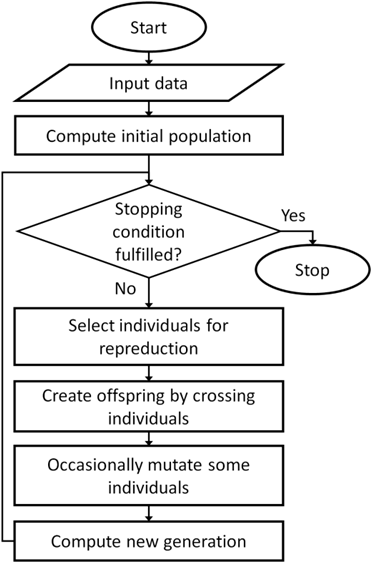
\includegraphics[width=0.48\textwidth]{wykresy/block.png}
\caption{Functional flowchart of~genetic algorithm}
\label{fig:block}
\end{figure}

As obvious from the~above algorithm, the~transition from one generation to~the~next consists of~four basic components \cite{mitchell1998introduction}:

\begin{itemize}
  \item[$\bullet$] \textbf{Selection:} Mechanism for selecting individuals (strings) for reproduction according to~their fitness (objective function value).
  \item[$\bullet$] \textbf{Crossover:} Method of~merging the~genetic information of~two individuals; if the~coding is~chosen properly, two good parents produce good children.
  \item[$\bullet$] \textbf{Mutation:} In real evolution, the~genetic material can by~changed randomly by~erroneous reproduction or other deformations of~genes, e.g. by~gamma radiation. In genetic algorithms, mutation can be~realized as~a~random deformation of~the~strings with a~certain probability. The positive effect is~preservation of~genetic diversity and, as~an~effect, that local maxima can be~avoided.
  \item[$\bullet$] \textbf{Sampling:} Procedure which computes a~new generation from the~previous one and its offspring.
\end{itemize}

Compared with traditional continuous optimization methods, such as~Newton, quasi-Newton or gradient descent methods, we can state the~following significant differences \cite{fletcher2013practical}:

\begin{enumerate}
  \item While almost all conventional methods search from a~single point, GAs always operate on~a~whole population of~points (strings). This contributes much to~the~robustness of~genetic algorithms. It improves the~chance of~reaching the~global optimum and, vice versa, reduces the~risk of~becoming trapped in~a~local stationary point.
  \item Normal genetic algorithms do not use any auxiliary information about the~objective function value such as~derivatives. Therefore, they can be~applied to~any kind of~continuous or discrete optimization problem. The only thing to~be done is~to~specify a~meaningful decoding function. 
  \item GAs use probabilistic transition operators while conventional methods for continuous optimization apply deterministic transition operators. More specifically, the~way a~new generation is~computed from the~actual one has some random components.
\end{enumerate}

